% !TEX encoding = UTF-8 Unicode
%!TEX root = thesis.tex
% !TEX spellcheck = en-US
%%=========================================



\chapter{Background}

\section{Augmented Reality}

\section{Neuro stuff}

\subsection*{Waxholm Space Atlas}\label{chap:ratbrain}

https://www.nitrc.org/projects/whs-sd-atlas
\begin{itemize}
    \item What is a atlas
    \item WHS and ratbrain is open, used and developed by NTNU St Olavs and UiO 
    \item Waxholm Space Atlas of the Sprague Dawley Rat Brain 
\end{itemize}

    % \caption{Waxholm Space in a rat brain with axis through origin \citep{WaxholmRatBrain2014}}
This brain model has been captured and manually delineated\footnotemark by a collaboration between research groups at the University of Oslo and NTNU.

\footnotetext{Delineation refers to the process of clearly defining different structures in the brain into separate namable parts.}

\noindent From \citet{WaxholmSpace2011}: 

\noindent The coordinate system for WHS is defined as a continuous Cartesian system with the origin in the brain determined by
\begin{wrapfigure}{r}{0.30\textwidth} 
    \centering
    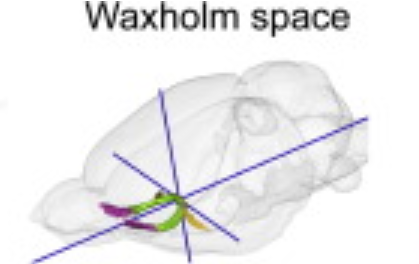
\includegraphics[width=0.25\textwidth]{fig/waxholmspace}
    \label{waxholmspace}
\end{wrapfigure}
\begin{itemize}
    \item the anterior commissure (AC) at the intersection between the mid-sagittal plane,
    \item a coronal plane passing midway (rostro-caudal) through the anterior and posterior branches of AC, and
    \item a horizontal plane passing midway through the most dorsal and ventral aspect of the AC.
\end{itemize}




\section{Related work}

\subsection*{HoloAnatomy}

\subsection*{Insight Heart}

\subsection*{SphenoBlock?}

\subsection*{Noe HoloCare stuff?}

